

\chapter{The muon}

\section{Muon history}

Muons were discovered by Carl David Anderson and his student Seth Neddermeyer at Caltech in 1936 while they were working on cosmic rays. They observed that certain particles had a much more strongly curved trajectory in their cloud chamber, than electron but less than protons. They were curving in the same direction as electrons meaning they had the same charge. They were initially mistaken for Yukawa's pion which supposedly mediated the strong interaction but was discovered not to have the right properties as it didn't interact strongly as it could traverse thick plates of metal unhindered. Heisenberg and Euler made the first computation of its lifetime in 1938, through the decreasing intensity as a function of travel distance. In 1947, Powell, Lattes, Muirhead and Ochialini used emulsion plates to discover two different ``mesons'': the \Ppi-meson and the \Pmu-meson (which was later revealed to be quite different from his counterpart).

\section{Muon production from pion decays}

Pions are the lightest hadron and thus can only decay electroweakly, they are, as $\Pquark\APquark$ with antiparallel spins, spinless bound-states. Since they can only decay to fermions, which have spin $\frac{1}{2}$, only even-number-body-decays are allowed by angular momentum conservation laws. In addition, because of flavour conservation laws, leptons need to be produced as pairs or together with a(n) (anti)neutrino. An example pion decay is given in Figure \ref{fig:pidec}.


\begin{figure}[htbp]
\centering
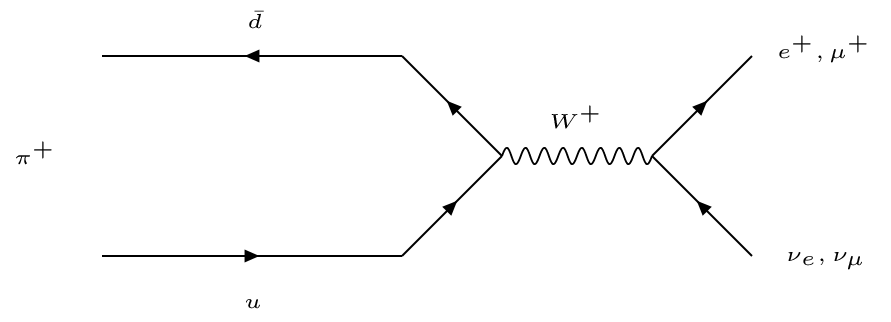
\includegraphics[width=0.7\linewidth]{./fig/pideac.png}
\caption{Positive pion decay.}
\label{fig:piedec}
\end{figure}

There are thus channels available for pions to decay:

\begin{equation*}
\Ppiplus \rightarrow \APelectron \Pnue \text{;\hspace{3cm}}\Ppiminus \rightarrow \Pelectron \APnue;
\end{equation*}

\begin{equation*}
\Ppiplus \rightarrow \APmuon \Pnum \text{;\hspace{3cm}}\Ppiminus \rightarrow \Pmuon \APnum.
\end{equation*}

This gives rise to the branching ratio:

\begin{equation}
R=\frac{\text{Rate}(\Ppi\rightarrow \Pe \Pnu)}{\text{Rate}(\Ppi\rightarrow \Pmu \Pnu)} = (1.230 \pm 0.004) \cdot 10^{-4}.
\end{equation}

Muon-channel decays are thus nearly 10000 times more likely than electron-channel decays. This might be surprising when looking at energy phase space consirations: the muon being around 207 times heavier than the electron, the phase space would thus be:

\begin{equation}
R_{\text{phase-space}}=\frac{1-\big(\frac{m_{\Pe}}{m_{\Ppi}}\big)^2}{1-\big(\frac{m_{\Pmu}}{m_{\Ppi}}\big)^2} \simeq 2.35.
\end{equation}

with $m_{\Ppi} = 273 m_{\Pe}$.

This wrong prediction is due to the lack of account taken from \textit{V-A Coupling}, the combination of a vector (such as flight direction) and an axial vector (such as momentum) in the weak decay. This requires a new quantum number to be introduced: \textit{Helicity H}, which is defined as the projection of spin on momentum:

\begin{equation*}
H\doteq \vec{s}\cdot \hat{p} \text{\hspace {1cm} with \hspace{1cm}} \hat{p}=\frac{\vec{p}}{|\vec{p}|}.
\end{equation*}

Helicity  expectation and alignement value are defined by:

\begin{equation*}
\Braket{H}\doteq\pm\frac{v}{c}.
\end{equation*}

With the expectation taking positive values for particles (\Pelectron, \Pmuon,\Pnue,\Pnum) and negatives ones for antiparticles (\APelectron,\APmuon,\APnue,\APnum). It should be noted that in the Standard Model, only \text{left-handed} ($\Braket{H}=-1$, spin and momentum antiparallel) neutrinos and thus only \textit{right-handed} ($\Braket{H}=+1$, spin and momentum parallel) antineutrinos. Neutrinos can be seen as practically massless and thus always travelling at the speed of light. This implies, through momentum and angular momentum conservation, pions can only decay in certain configurations such as that shown in Figure \ref{fig:helipi}.

\begin{figure}[htbp]
\centering
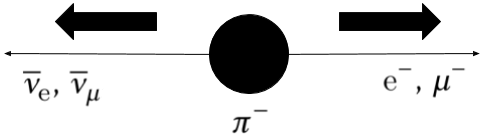
\includegraphics[width=0.7\linewidth]{./fig/helipi2.png}
\caption{Spin and momentum in a negative pion's decay, as seen in the pion's rest frame.}
\label{fig:helipi}
\end{figure}

Since the pion is spinless, the neutrino and charged fermion need to have opposite spin, since antineutrinos can only have right-handed helicity, the muon is emitted with right-handed helicity. However, only left-handed particles participate in the weak interaction. This can be seen in the right-handed helicity solution of the Dirac equation:

\begin{equation}
u_{\uparrow}=N\begin{pmatrix} \cos{\frac{\theta}{2}} \\ e^{i\phi}\sin{\frac{\theta}{2}} \\ \frac{|\vec{p}|}{E+m}\cos{\frac{\theta}{2}} \\ \frac{|\vec{p}|}{E+m}e^{i\phi}\sin{\frac{\theta}{2}} \end{pmatrix}.
\end{equation}

The left-handed chirality projector is given by:

\begin{equation}
P_{\text{L}}=\frac{1}{2}(1-\gamma^5)=\frac{1}{2} \begin{bmatrix} 1 & 0 & -1 & 0 \\
0 & 1 & 0 & 1 \\
-1 & 0 & 1 & 0 \\
0 & -1 & 0 & 1 \end{bmatrix}.
\end{equation} 

with, when applied to the spinor yields:

\begin{equation}
P_{\text{L}}u_{\uparrow}=\frac{N}{2}\Big(1-\frac{|\vec{p}|}{E+m}\Big)u_{\text{L}}.
\end{equation} 

which tends to zero in the limit $m<<E$, while

\begin{equation}
P_{\text{R}}u_{\uparrow}=\frac{N}{2}\Big(1+\frac{|\vec{p}|}{E+m}\Big)u_{\text{R}}.
\end{equation}

tends to $u_{\text{R}}$ in the limit $m<<E$. This leads to

\begin{equation}
u_{\uparrow}=P_{\text{R}}u_{\uparrow} + P_{\text{L}}u_{\uparrow} = \frac{1}{2}\Big(1+\frac{|\vec{p}|}{E+m}\Big)u_{\text{R}} + \frac{1}{2}\Big(1-\frac{|\vec{p}|}{E+m}\Big)u_{\text{L}}.
\end{equation}

in the limit $E>>m$, the right-handed chiral and helicity states are identical as expected. Even though only left-handed chiral particles participate in the weak interaction, the right-handed contribution isn't necessarily zero. The matrix element is expected to be proportional to the left-handed chiral component of the right-handed helicity fermion spinor:

\begin{equation}
\text{M}_{fi} \propto \frac{1}{2} \Big(1-\frac{|\vec{p}|}{E+m}\Big) = \frac{m}{m_{\Ppi}+m} .
\end{equation}

The calculation of the branching ratio

\begin{equation}
R=\frac{P(\Ppi\rightarrow \Pe \Pnu)}{P(\Ppi\rightarrow \Pmu\Pnu)}\simeq \frac{m_{\Pe}^2}{m_{\Pmu}^2}\frac{(1-\frac{m_{\Pe}^2}{m_{\Ppi}^2})^2}{(1-\frac{m_{\Pmu}^2}{m_{\Ppi}^2})^2} \simeq 1.283 \cdot 10^{-4}.
\end{equation}

Which is in good agreement with experimental observations. For this measurement, it is necessary that muon in the pion rest-frame be entirely left-handed. The Lorentz transform into the Lab-frame allows for this in this experiment.

\section{Muon polarization in cosmic rays}

In this experiment, muons will be stopped in a \SI{25}{mm} thick copper plate. If other present materials are accounted for, such as the lead shielding, concrete ceilling and \SI{20}{\km}, only ``slow'' muons, with an energy estimated to be of $\sim\SI{609}{MeV}$ are actually stopped in the copper. While this might be an estimate, Figure \ref{fig:mupol} demonstrates the relative constance of polarization at energies between \SI{300}{\MeV} and \SI{900}{\MeV}.

\begin{figure}[htbp]
\centering
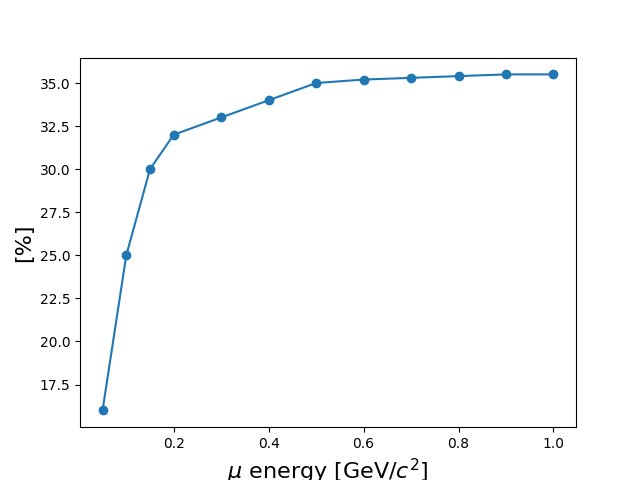
\includegraphics[width=0.7\linewidth]{./fig/muonpol.png}
\caption{Muon polarization as a function on energy.}
\label{fig:mupol}
\end{figure}

Muons of such energies can be created in two different ways (in the following, positive muons will be looked at):

\begin{itemize}

\item They can be produced in \SI{616}{\MeV} pions and are then emitted in the direction of flight, with negative helicity and upward-facing spin (Figure \ref{sfig:spindeca}).

\item They can be produced in \SI{1058}{\MeV} pions and are then emitted against the direction of flight, with positive helicity and downward-facing spin (Figure \ref{sfig:spindecb}).

\end{itemize}

\begin{figure}[htbp]
\centering
\caption{Muon polarization as a function on energy.}
\end{figure}

\begin{figure}[htbp]
  \centering
   \begin{subfigure}[t]{0.49\linewidth}
  \centering
   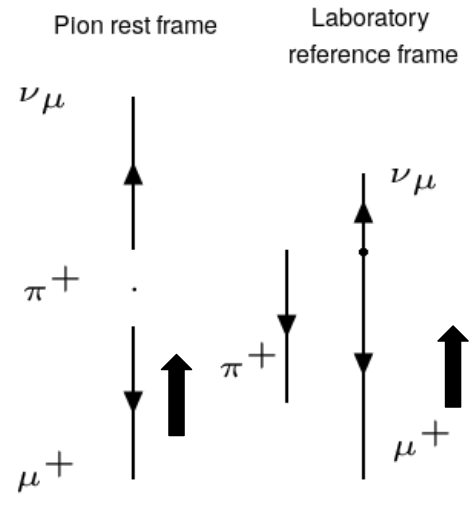
\includegraphics[width=0.7\linewidth]{./fig/spindecaa.png}
  \caption{}
\label{sfig:spindeca}
  \end{subfigure}
 \begin{subfigure}[t]{0.49\linewidth}
  \centering
   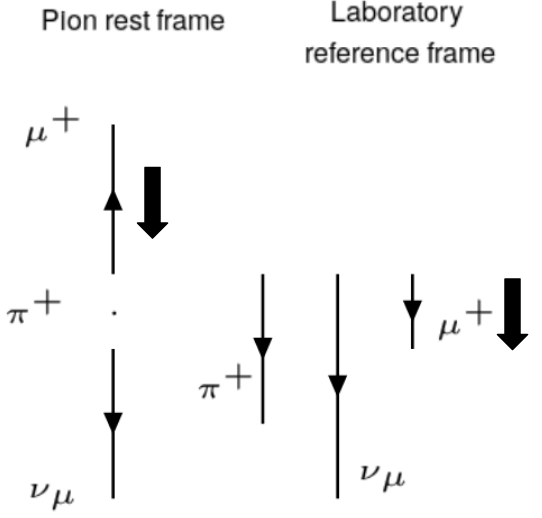
\includegraphics[width=0.7\linewidth]{./fig/spindecbb.png}
  \caption{}
  \label{sfig:spindecb}
  \end{subfigure}
  \caption{Production of \SI{609}{\MeV} in cosmic radiation with (a) negative helicity and (b) positive helicity.}%
  \label{fig:spindec}
\end{figure}

With a uniform pion energy distribution, it was first impossible to observe polarized muons. At the aforementionned energy ranges however, the pion abundance as a function of energy $N(E)$ can be seen to display the following behaviour:

\begin{equation}
N(E) \mathrm{d}E \sim E^{-1.4}\mathrm{d} E.
\end{equation}

Thus the ratio of muons with positive helicity $N(\downarrow\uparrow)$ to those with negative helicity $N(\uparrow\uparrow)$ is:

\begin{equation}
\frac{N(\downarrow\uparrow)}{N(\uparrow\uparrow)}=\frac{616^{-1.4}}{1058^{-1.4}}\simeq \frac{2.15}{1}.
\end{equation}

An excess of muons with negative helicity is thus of polarization is expected. The polarization $P$ is defined as:

\begin{equation}
P\doteq \frac{N(\downarrow\uparrow)-N(\uparrow\uparrow)}{N(\downarrow\uparrow)+N(\uparrow\uparrow)}.
\end{equation}

It is thus expected to find a muon polarization of about $37\%$.

\section{Muon decays}

Muons decay with an average lifetime of $2.2 \cdot 10^{-6}\si{\second}$ into the lighter flavoured lepton, the electron. Since muons are stopped in copper and that the process is different for positive and negative muons, both processes will be treated separately.

\subsection{The decay of free \APmuon}

Positive muons remain in the free interstices and can thus decay like free muons. In order to preserve lepton number, the following decay takes place:

\begin{equation*}
\APmuon \rightarrow \APelectron + \Pnue + \APnum.
\end{equation*}

As a three-body decay, the positron's momentum spectrum is continious, however, due to the parity-violating nature of the weak interaction, an assymetry in the positron's angular distribution can be found as shown in Figure \ref{fig:angassy}

\begin{figure}
\centering
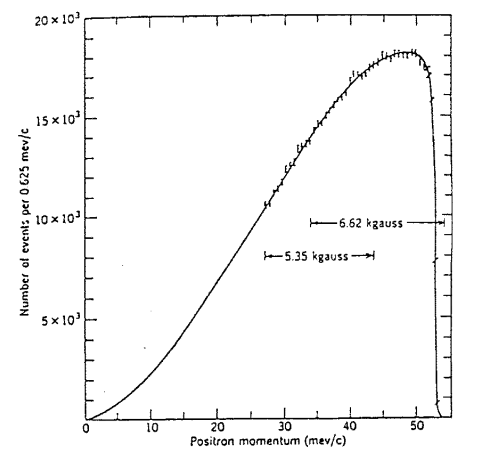
\includegraphics[width=0.5\linewidth]{./fig/posangas.png}
\caption{Final state positron from muon decays momentum spectrum.}
\label{fig:angassy}
\end{figure}

For the transition probability $W$ for the solid angle $\Omega$:

\begin{equation}
\label{eq:e413}
\mathrm{d}W=\frac{G_{\text{F}}^2m_{\Pmu}^5c^4}{192\pi^3\hbar^7}\big[2\epsilon^2(3-2\epsilon) \big] \Bigg[1+\frac{1-2\epsilon}{3-2\epsilon} \cos{\Theta} \Bigg] \Bigg[ \frac{1-n_{\Pe}s_{\Pe}}{2}\Bigg]\mathrm{d}\epsilon \frac{\mathrm{d}\Omega}{4\pi},
\end{equation}

with $\epsilon = \frac{E_{\Pe}}{E_{\text{max}}}$, $E_{\text{max}} = \frac{1}{2m_{\Pmu}c^2}$ and $\Theta$ the angle between the muon's spin and the positron's momentum. The first block between brackets provides the positron momentum spectrum, the second provides the angular distribution and the third represents the positron helicity in the V-A description. The third block can be approximated with $\frac{v_{\text{pos}}}{c} \sim 1$ and thus can be neglected. For the number of positron emitted at an angle $\Theta$ one can write:

\begin{equation}
N(\Theta)\sim 1+ a\cos{\Theta} \text{ with the assymmetry factor } a=\frac{1-2\epsilon}{3-2\epsilon}.
\end{equation}

The average assymmetry over all energies can be integrated from Equation \ref{eq:e413}:

\begin{equation}
N(\epsilon) \sim \int_0^1 \big[2\epsilon^2(3-2\epsilon) \big] \Bigg[1+\frac{1-2\epsilon}{3-2\epsilon} \cos{\Theta} \Bigg] \mathrm{d}\epsilon \implies N(\Theta)\sim 1 + \frac{1}{3}\cos{\Theta}.
\end{equation}

This corresponds to an assymmetry of $\sim 33\%$. This is illustrated in Figure \ref{fig:emassy}.

\begin{figure}[htbp]
\centering
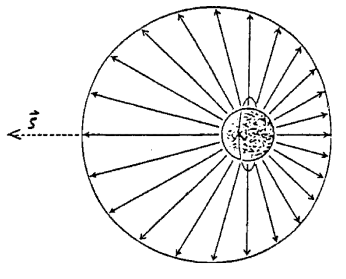
\includegraphics[width=0.7\linewidth]{./fig/emassy.png}
\caption{Illustration of positron angle emission in muon decays. The length of the arrow is proportional to the emission probability for that angle.}
\label{fig:emassy}
\end{figure}

In order for them to be detected, the positrons first need to exit the copper plate which, depending on their emission angle and the decay vertex position, requires a minimal energy of \SI{30}{\MeV}. This leads to an assymmetry factor $a=0.38\pm0.04$ \cite{Heel}. The oberserved assymmetry in this measurement also depends on the Polirization $P$ of the muon:

\begin{equation}
\label{eq:larg}
N(\Theta)\sim1+aP\cos{\Theta}.
\end{equation}

The last remaining unknown if the muon's lifetime $\tau_{\Pmu}$. Integrating Equation \ref{eq:e413} over space and energy provides the transition probability $W$ which is nothing else than the \textit{inverse lifetime}:

\begin{equation}
W=\frac{G^2_{\text{F}}2m_{\Pmu}^5c^4}{192\pi^3\hbar^7}=\frac{1}{\tau_{\Pmu}}.
\end{equation}

Litterature places this lifetime at $2.197\cdot 10^{-6} \si{\second}$. By measuring the muon's lifetime, one can thus also obtain a value of Fermi's coupling constant $G_{\text{F}}$.

\section{Nuclear capture of negative muons}

As opposed to antimuons, muons are mostly captured by nuclei. This process takes place after the muons are decelerated through ionization processes from the speed of light to approximately $6\cdot10^{-3}c\text{ }(\simeq\SI{2}{\kilo\electronvolt})$ in $\sim \SI{e-9}{\second}$. They are then captured by the atom in around $\SI{e-13}{\second}$. The muon then cascades through the K-Shell in a time proportionnal to $Z^4$ with Z the number of protons in the nucleus. This time ranges from $\SI{e-9}{\second}$ for Uranium to $\SI{e-17}{\second}$ for Hydrogen. As the muon and electrons are otherwise identical particles, the orbit radius of muon-shells is calculated in the same way as that of electrons except for one thing: due to the 207 mass-factor difference between electrons and muons, the muon's Bohr radius is 207 times smaller which implies a much more overlapping between the nucleus' and muon's wavefunctions. This implies a high probability of nuclear capture through the process:

\begin{equation}
\Pmuon + \Pproton \rightarrow \Pneutron + \Pnum.
\end{equation}

Thus the total decay probability $W$ is calculated from the sum of the initial probability $W_{\text{i}}$ and the decay probability $W_{\text{d}}$ in the K-Shell: $W=W_{\text{i}}+W_{\text{d}}$. As such, the lifetime of negative muons $\tau_-$ is calculated as:

\begin{equation}
\label{eq:Wtau}
\frac{1}{\tau_-}=\frac{1}{\tau_{\text{d}}}+\frac{1}{\tau_{\text{i}}},
\end{equation}

with $\tau_{\text{d}}=\frac{1}{W_{\text{d}}}$ and $\tau_{\text{i}}=\frac{1}{W_{\text{i}}}$. The probability $W_{\text{i}}$ scales as:

\begin{equation}
\label{eq:Wzeff}
W_{\text{i}}=W_{\text{d}}\Big( \frac{z_{\text{eff}}}{z_0}\Big)^4, \text{ with } z_0=10.8.
\end{equation}

$z_{\text{eff}}$ is here the effective nuclear charge which for copper ($Z=29$) is:

\begin{equation}
z_{\text{eff}}=z(1+(\frac{z}{42})^{1.47})^{\frac{-1}{1.47}}\simeq 21.
\end{equation}

Assuming that the decay probability of the negative muon in a K-Shell is identical to that of a free muon ($\frac{1}{\tau_{+}}$), then according to Equations \ref{eq:Wtau} and \ref{eq:Wzeff}, the average lifetime $\tau_-$ of negative muons:

\begin{equation}
\tau_-=\tau_+\frac{z_0^4}{z_0^4+z_{\text{eff}}^4}.
\end{equation}

For copper this is roughly $\tau_-=\SI{144}{\nano\second}$. For nuclei with low charges, the difference in the average lifetimes is small (for Carbon, $\tau_-=(0.1635 \pm 0.0024)\text{ }\si{\micro\second}$). \Pmuon is in this measurement measured indirectly through the detection of the $\beta$ from excited Nickel nuclei which arise from copper nuclei:

\begin{equation}
\begin{split}
\Pproton+\Pmuon \rightarrow&\Pneutron+\Pnum \\
(\text{Cu}+\Pmuon\rightarrow &\text{Ni}^*+\Pnum) \\
&\hookrightarrow\text{Ni}^*\rightarrow \text{Cu} + \Pelectron + \APnue \\
&\hspace{0.5cm}(n\rightarrow\Pproton+\Pelectron+\APnue)
\end{split}
\end{equation}

Since this process is quite fast, the electron is seen at about the same time as the muon.


\section{Muon magnetic moment}

The muon, as a fermion (particle with $s=\frac{1}{2}$) and charge $e$ has a magnetic moment:

\begin{equation}
\mu_{\Pmu}=\frac{e\hbar}{2m_{\Pmu}},\text{ in litterature, } \mu_{\Pmu}=\SI{4.49045e-26}{\joule\per\tesla}.
\end{equation}

In a B-field with flux-density $B$, the muon spin precesses with a \textit{Larmor-Frequency} $\omega_{\text{L}}$:

\begin{equation}
\label{eq:larm}
\omega_{\text{L}}=g\frac{eB}{2m_{\Pmu}}=g\frac{\mu_{\Pmu}B}{\hbar}.
\end{equation}

For our purpose, the muon's $g-Factor$ can be approximated to $g=2$ ($g-2=11659208.9\pm_{\text{stat}}5.4\pm_{\text{syst}}3.3\cdot 10^{-10}$ \cite{Tanabashi:2018oca}). The Larmor Frequency is then approximately $\SI{85.14}{\kilo \hertz \per \gauss}$. In particular, because of their spin, emitted positrons precesses in the same direction as their emission direction.


